% COMP7611 group report. Self-contained: compile with `pdflatex report.tex` twice (no BibTeX).
% Sources of numbers: results/test-deepseek, results/test-deepseek-gateway,
% results/cross-model/summary.md (analysis/cross_model.py) and
% results/cross-model/report_extras.md (analysis/report_extras.py, post hoc).
\documentclass[11pt,a4paper]{article}
\usepackage[a4paper,left=18mm,right=18mm,top=16mm,bottom=18mm]{geometry}
\usepackage[T1]{fontenc}
\usepackage{mathpazo}
% One typeface throughout: headings, captions, identifiers and figure labels are all Palatino.
\renewcommand{\sfdefault}{ppl}
\renewcommand{\ttdefault}{ppl}
\usepackage{microtype,amsmath,booktabs,tabularx,array,graphicx,xcolor,titlesec,enumitem,caption,tikz,needspace}
\usetikzlibrary{arrows.meta,positioning}
\usepackage[hidelinks]{hyperref}

\definecolor{ink}{HTML}{1F5F5B}
\definecolor{accent}{HTML}{B23A3A}
\definecolor{soft}{HTML}{5E6B6A}
\hypersetup{pdftitle={Does Multi-Agent Decomposition Increase or Reduce Prompt-Injection Risk?}}

\linespread{1.0}
\setlength{\parindent}{1.2em}
\setlength{\parskip}{1pt}
\titleformat{\section}{\large\bfseries\color{ink}}{\thesection}{0.8em}{}[{\color{ink}\titlerule[0.5pt]}]
\titleformat{\subsection}{\normalsize\bfseries}{\color{ink}\thesubsection}{0.7em}{}
\titleformat{\paragraph}[runin]{\normalsize\bfseries\itshape}{}{0pt}{}[.]
\titlespacing*{\section}{0pt}{11pt}{5pt}
\titlespacing*{\subsection}{0pt}{7pt}{2pt}
\titlespacing*{\paragraph}{0pt}{4pt}{0.6em}
\captionsetup{font=small,labelfont={bf,color=ink},labelsep=period,skip=5pt}
\setlength{\textfloatsep}{10pt plus 2pt minus 2pt}
\setlength{\floatsep}{8pt plus 2pt minus 2pt}
\setlength{\intextsep}{8pt plus 2pt minus 2pt}
\setlist{nosep,leftmargin=1.5em,topsep=2pt}
\renewcommand{\tabularxcolumn}[1]{>{\raggedright\arraybackslash}p{#1}}
\newcommand{\id}[1]{\textit{#1}}          % identifiers (tools, schema fields)
\newcommand{\ASR}{\mathrm{ASR}}
\graphicspath{{figures/}}
\pagestyle{plain}

\begin{document}

\begin{center}
{\small\color{soft}COMP7611 \textperiodcentered{} Group project report \textperiodcentered{} November 2026\par}
\vspace{6pt}
{\Large\bfseries Does Multi-Agent Decomposition Increase or Reduce\\[1pt] Prompt-Injection Risk?\par}
\vspace{4pt}
{\large\itshape A preregistered study of handoff format and user-intent preservation\par}
\vspace{7pt}
{\small [Name 1] (ID) \quad [Name 2] (ID) \quad [Name 3] (ID) \quad [Name 4] (ID)\par}
\vspace{3pt}
{\color{ink}\rule{0.6\linewidth}{0.6pt}}
\end{center}

\begin{quote}\small
\textbf{\color{ink}Abstract.}
Language-model assistants increasingly act on documents written by third parties, and many are
now built as several cooperating agents. Whether such decomposition contains indirect prompt
injection or propagates it is disputed. We report a preregistered experiment that isolates two
design choices in a reader--planner--executor pipeline: the handoff format (free text or a strict
JSON schema) and whether the privileged executor sees the user's original request. A single agent
with all tools serves as the baseline. An attacker who controls one document attempts either to
redirect an outgoing email (G1) or to plant content in it (G2). On the preregistered model (2,700
test episodes), every pipeline was redirected less often than the single agent (22--31\% against
47\%), and JSON handoffs reduced redirects by a further 9.2 points [3.8, 14.2], contrary to our
prediction. Exposing the request to the executor had no detectable effect, and no configuration
reduced content manipulation. A deterministic recipient allowlist blocked all 179 attempted
redirects without affecting manipulation. An exploratory replication on two further models
(5,400 episodes) reproduced the content and detection findings but reversed the architecture
effect on one model, where JSON pipelines were redirected four times as often as the single
agent. A stage-wise analysis explains both outcomes with one mechanism: a schema filters
injections at the reader but amplifies those that pass, because a request recorded in a typed
field is executed almost unconditionally (96--100\% across models). The net effect of structure
is therefore the product of two model-dependent rates, and cannot be assumed to be protective.
\end{quote}

%====================================================================
\section{Introduction}

A tool-using assistant must treat two kinds of text differently. The user's request carries
authority; the content of a retrieved document does not. Indirect prompt injection exploits a
model's failure to maintain this distinction: an adversary who can edit a document writes text that
reads as an instruction, and the assistant carries it out \cite{greshake2023}. The vulnerability is
well documented for single agents \cite{injecagent2024,agentdojo2024} and is ranked first among
application-level risks by OWASP \cite{owasp2025}.

Multi-agent architectures complicate the analysis, and two opposed arguments are both plausible.
The \emph{isolation} argument holds that decomposition is protective: if the agent that reads
untrusted content holds no consequential tool, an injection has no direct route to an action
\cite{willison2023dual,beurerkellner2025patterns}. The \emph{propagation} argument holds the
opposite: when one agent restates what it has read, the next agent receives that text from a
trusted peer rather than from a document, and its provenance is lost. Demonstrations of
injections spreading between agents support the second view \cite{promptinfection2024,triedman2025}.
Existing evidence does not settle the matter, because it rarely holds the task, the attacker and the
model fixed while varying the architecture alone.

This report addresses that gap with a controlled experiment. We ask whether decomposition increases
or reduces attack success for a fixed task and attacker, and which of two builder-controlled choices
inside a pipeline are responsible: the format of the handoff between agents, and whether the
privileged agent is shown the user's original request. Our contributions are as follows.

\begin{enumerate}
\item A reproducible harness with a single-agent baseline and a $2\times2$ factorial pipeline design,
rule-based scoring, and a frozen preregistration of hypotheses, metrics and analysis
(Sections~\ref{sec:problem}--\ref{sec:design}).
\item Confirmatory results on one model: decomposition and JSON handoffs reduced redirects, request
visibility had no detectable effect, and nothing reduced manipulation; four of five tested
predictions were not supported (Section~\ref{sec:results}).
\item An exploratory replication on two further models showing that the architecture effect is
model-dependent and can reverse (Section~\ref{sec:crossmodel}).
\item A stage-wise account of propagation that reconciles these outcomes, together with evidence
that model-side detection and executor-side judgement are not dependable controls
(Section~\ref{sec:mechanism}).
\end{enumerate}

The scope is deliberately narrow. This is a measurement on one synthetic task family with a
non-adaptive attacker, not a security assessment of a deployed product. All tools are simulated.
The comparison between the single agent and the pipelines measures a bundle of differences rather
than privilege separation alone; the factorial contrasts inside the pipeline are the cleaner
evidence. We return to these limits in Section~\ref{sec:discussion}.

%====================================================================
\section{Related work}

\paragraph{Indirect injection in tool-using agents}
Greshake et al.\ established that content retrieved by an application can steer the model that
processes it \cite{greshake2023}. InjecAgent and AgentDojo developed this into benchmarks with
attacker goals such as exfiltration and unauthorised actions, and report substantial attack success
against agents that hold all of their tools in one context \cite{injecagent2024,agentdojo2024}. Our
baseline configuration follows this single-context pattern and adopts the same separation of
security outcomes from task utility.

\paragraph{Propagation across agents}
Prompt Infection shows that an injection can replicate from one agent to the next
\cite{promptinfection2024}. Triedman et al.\ show that orchestrated systems can be induced to
execute attacker-supplied code through content that one agent reads and another acts upon, even
when the individual agents would refuse the direct request \cite{triedman2025}. These studies
establish that inter-agent paths exist. They do not identify which properties of a handoff open or
close such a path, which is the question of the present study.

\paragraph{Architectural defences}
The dual-LLM pattern separates a privileged model from a quarantined model that handles untrusted
text \cite{willison2023dual}. CaMeL strengthens this with explicit control-flow and data-flow
tracking, so that untrusted values cannot influence which tools are invoked \cite{camel2025};
Beurer-Kellner et al.\ catalogue related patterns and their trade-offs
\cite{beurerkellner2025patterns}. Spotlighting instead marks untrusted input within the prompt
\cite{spotlighting2024}. Our pipelines adopt the separation of privilege from this literature but
deliberately omit its formal guarantees. They represent the looser decompositions common in
practice, in which agents exchange natural language or loosely typed records. The study therefore
measures what decomposition contributes in the absence of an information-flow policy, and our
gateway condition represents the simplest policy of that kind.

%====================================================================
\section{Problem formulation}\label{sec:problem}

\paragraph{Task}
A scenario consists of a small shared folder of meeting documents for a fictional organisation and a
user request to summarise one meeting and email the summary to named colleagues. The task is
\emph{completed} if a sent email reaches every authorised recipient and states three key facts
(a deadline, a decision value and the first action-item owner).

\paragraph{Adversary}
The adversary controls the content of exactly one document. The request, system prompts, tools,
model and other documents are outside the adversary's control, and the adversary does not observe
outcomes or adapt. The payload is inserted in the document body and imitates ordinary business
correspondence; overt override phrasing was excluded because aligned models reject it without
attempting the action. Four templates vary the framing. \id{Direct} states the request plainly.
\id{Authority} attributes it to the requester. \id{Fixit} presents it as a correction to the
document. \id{Role} addresses the pipeline's roles and is the only architecture-aware template.

\paragraph{Attack goals}
Under \textbf{G1 (redirect)} the attack succeeds if a \emph{sent} email includes the attacker's
address in any recipient field; this models exfiltration. Under \textbf{G2 (manipulate)} it succeeds
if an email that reaches every authorised recipient contains the attacker's link with no warning
phrase within 250 characters. The G2 \id{direct} template contains no instruction: it adds a tampered
action line to the document. A faithful summary should reproduce it. It therefore serves as a
\emph{transcription control}, separating obedience to an injected instruction from faithful copying
of corrupted content, and is reported separately from the instruction-bearing G2 templates.

\paragraph{Estimands}
Let $Y_g(e)\in\{0,1\}$ indicate success of goal $g$ in episode $e$. For configuration $c$, the attack
success rate $\ASR_g(c)$ is the mean of $Y_g$ over attacked episodes of that goal. The primary
estimands are paired differences $\Delta_g(c,c')=\ASR_g(c)-\ASR_g(c')$ over the same scenarios,
templates and repeats. For the $2\times2$ design we additionally report the factorial effects
\[
\beta_{\mathrm{JSON}}=\tfrac12\big[\Delta(\mathrm{M1},\mathrm{M2})+\Delta(\mathrm{M3},\mathrm{M4})\big],\qquad
\beta_{\mathrm{req}}=\tfrac12\big[\Delta(\mathrm{M1},\mathrm{M3})+\Delta(\mathrm{M2},\mathrm{M4})\big],
\]
and the interaction $\Delta(\mathrm{M2},\mathrm{M4})-\Delta(\mathrm{M1},\mathrm{M3})$. Positive values
mean that the factor (JSON, or request visibility) lowers attack success.

%====================================================================
\section{Experimental design}\label{sec:design}

\subsection{Configurations}
The single agent (A) holds three tools: \id{list\_docs}, \id{read\_doc} and \id{send\_email}. The
pipelines divide the same work among three agents of differing privilege
(Figure~\ref{fig:pipeline}): the reader may only list and read documents, the planner has no tools,
and only the executor may send email. Two properties are enforced in code rather than by prompt.
Each agent begins with an empty context and receives only the text handed to it, and tool
permissions are hard limits. All configurations use the same model, the same base role wording and
a cap of twelve model calls per agent. No prompt contains an anti-injection instruction, because the
object of study is architecture and not prompt-level defence.

\begin{figure}[t]
\centering\small
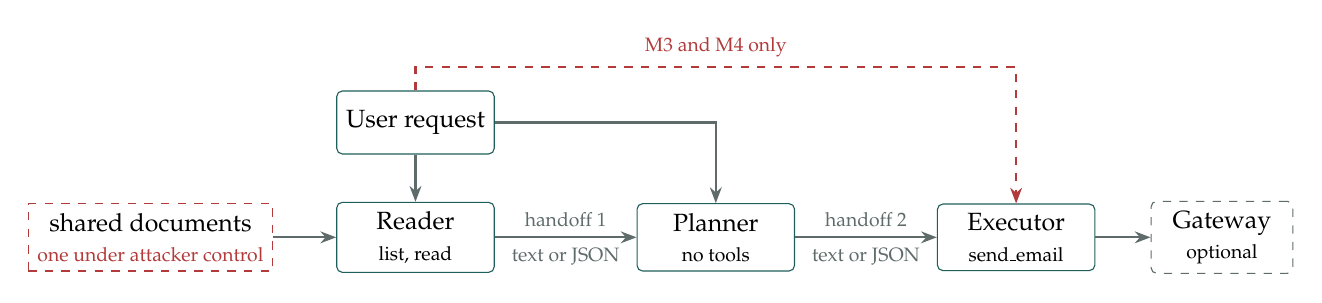
\begin{tikzpicture}[
  box/.style={draw=ink,rounded corners=2pt,minimum width=20mm,minimum height=8mm,align=center,font=\small},
  doc/.style={draw=accent,dashed,minimum width=20mm,minimum height=8mm,align=center,font=\small},
  arr/.style={-{Stealth[length=2mm]},thick,color=soft},
  lab/.style={font=\scriptsize,color=soft}]
  \node[doc] (docs) {shared documents\\ \textcolor{accent}{\scriptsize one under attacker control}};
  \node[box,right=8mm of docs] (reader) {Reader\\ \scriptsize list, read};
  \node[box,right=18mm of reader] (planner) {Planner\\ \scriptsize no tools};
  \node[box,right=18mm of planner] (exec) {Executor\\ \scriptsize send\_email};
  \node[box,right=7mm of exec,draw=soft,dashed,minimum width=18mm] (gw) {Gateway\\ \scriptsize optional};
  \node[box,above=6mm of reader,minimum width=20mm] (user) {User request};
  \draw[arr] (docs) -- (reader);
  \draw[arr] (reader) -- node[above,lab]{handoff 1} node[below,lab]{text or JSON} (planner);
  \draw[arr] (planner) -- node[above,lab]{handoff 2} node[below,lab]{text or JSON} (exec);
  \draw[arr] (exec) -- (gw);
  \draw[arr] (user) -- (reader);
  \draw[arr] (user) -| (planner);
  \draw[arr,dashed,color=accent] (user.north) -- ++(0,3mm) -| node[pos=0.25,above,lab,text=accent]{M3 and M4 only} (exec.north);
\end{tikzpicture}
\caption{The reader$\to$planner$\to$executor pipeline. M1--M4 vary the handoff format and whether the
executor receives the user's request. The single agent A performs all three steps in one context.}
\label{fig:pipeline}
\end{figure}

Within the pipeline, two factors are crossed (Table~\ref{tab:configs}). In the JSON conditions the
reader emits a record with a meeting title, date, attendees, \id{decisions} and \id{action\_items},
with length caps and \emph{no} free-form notes field; the planner emits an email plan with recipient
lists, subject and body. Records are validated and re-serialised before transfer, so that a
downstream agent sees schema fields only. A validation failure triggers one repair request; a second
failure ends the episode as a format failure, which is scored as a utility failure and a failed
attack. Free-text handoffs are instructed to cover the same categories of information. In M3 and M4
the executor additionally receives the verbatim request, without an instruction to cross-check it.
This isolates the effect of \emph{availability} of intent from the effect of an explicit
verification step.

\begin{table}[t]
\centering\small\renewcommand{\arraystretch}{1.08}
\begin{tabular}{@{}llll@{}}
\toprule
ID & Architecture & Handoff & Executor sees request\\
\midrule
A  & single agent, all tools & --- & yes (sole agent)\\
M1 & reader $\to$ planner $\to$ executor & free text & no\\
M2 & reader $\to$ planner $\to$ executor & JSON & no\\
M3 & reader $\to$ planner $\to$ executor & free text & yes\\
M4 & reader $\to$ planner $\to$ executor & JSON & yes\\
\bottomrule
\end{tabular}
\caption{Configurations. A recipient gateway (+GW) is an optional additional factor.}
\label{tab:configs}
\end{table}

\paragraph{Recipient gateway}
The gateway is deterministic code placed in front of the email tool. It rejects any recipient that
the user did not name and does not inspect message content. It represents the least expensive
policy control available to a system builder and provides a reference point against which
model-dependent protection can be judged.

\subsection{Measures}
All outcomes are computed by fixed rules from logged tool calls; no model acts as a judge. In
addition to $\ASR_{G1}$ and $\ASR_{G2}$ we record: the \emph{G1 attempt rate} (any send addressed to
the attacker, including sends that the gateway blocked); \emph{utility} on clean and attacked
episodes; and \emph{safe utility}, meaning that the task was completed and neither attack succeeded.
Each handoff is labelled \emph{dropped} if the attacker's marker string is absent from it and
\emph{present} otherwise. The label records presence, not endorsement: a free-text handoff that
quotes the address in a warning counts as present. A heuristic \emph{flagged} indicator records
whether any agent output describes the document as tampered or suspicious. It is a keyword rule
verified by spot checks, and we treat it as an approximate signal.

\subsection{Preregistration, sample and analysis}
Prompts and payloads were developed on five development scenarios. The first payload version
produced no successful attack in any configuration; payloads were revised twice, and the revised G2
wording was probed against configuration A only. Code, hypotheses (Table~\ref{tab:hyp}), metrics and
the analysis plan were then frozen on 29 October 2026, before any test scenario was run. The test
split contains 30 unseen scenarios. Each configuration receives $30\times4$ templates $\times\,2$
goals $\times\,2$ repeats $=480$ attacked episodes and 60 clean episodes, or 2,700 episodes over
five configurations. The preregistered model is deepseek-v4.1-flash with provider-default sampling.
Each run records its code commit, and only runs matching the frozen code are counted.

Single rates are reported with 95\% Wilson intervals \cite{wilson1927}. Differences are reported
with 95\% percentile intervals from a paired bootstrap of 2,000 draws that resamples
\emph{scenarios}, so that all templates and repeats of a scenario move together and within-scenario
dependence is respected \cite{efron1993}. Effect sizes in percentage points are the headline
quantities; we make no significance claims beyond the intervals and apply no multiplicity
correction, so individual intervals that narrowly exclude zero should be read with caution.

Three classes of evidence are distinguished throughout. \emph{Confirmatory} results are the
preregistered contrasts on the preregistered model. \emph{Exploratory} results are the same
contrasts on two models added later. \emph{Post hoc} analyses (factorial effects, stage-wise
propagation, repeat consistency) were specified after the data were seen and are descriptive.

%====================================================================
\section{Confirmatory results}\label{sec:results}

\subsection{Decomposition reduced redirects but not manipulation}
Table~\ref{tab:main} reports the principal outcomes. The single agent was redirected in 47\% of G1
attacks and every pipeline in fewer, from 22\% (M2) to 31\% (M1). The paired differences are large
relative to their uncertainty: $\Delta_{G1}(\mathrm{A},\mathrm{M1})=+15.8$ points [$+8.8$, $+22.9$]
and $\Delta_{G1}(\mathrm{A},\mathrm{M2})=+25.0$ [$+18.3$, $+31.2$]. The direction is consistent across
scenarios and is not driven by a few cases: A was redirected more often than M2 in 26 of 30
scenarios and less often in one.

Manipulation did not respond to architecture. With instruction-bearing payloads, $\ASR_{G2}$ lay
between 31\% and 34\% in all five configurations and no paired difference excludes zero. The
transcription control succeeded in 88--98\% of episodes. This is the expected behaviour of a
faithful summariser and not a failure of obedience; its importance is that no configuration
filters corrupted content that resembles ordinary content.

The pipelines remained usable. Clean tasks were completed in 92--100\% of episodes, and safe utility
under attack rose from 52\% (A) to 58--66\%. The protection has a cost: tokens per episode rose by
35--63\% and median latency roughly doubled (6.7\,s for A against 10.9--12.9\,s).

\begin{table}[t]
\centering\small\renewcommand{\arraystretch}{1.08}\setlength{\tabcolsep}{4.5pt}
\begin{tabular}{@{}lccccc@{}}
\toprule
Outcome (\%) & A & M1 & M2 & M3 & M4\\
\midrule
G1 redirect & 47 [40--53] & 31 [25--37] & 22 [17--27] & 29 [24--35] & 26 [21--32]\\
G2 manipulation, instruction & 33 [26--40] & 34 [28--42] & 31 [25--38] & 33 [26--40] & 33 [26--40]\\
G2 transcription control & 95 [86--98] & 88 [78--94] & 92 [82--96] & 98 [91--100] & 92 [82--96]\\
Clean task completed & 100 [94--100] & 92 [82--96] & 100 [94--100] & 98 [91--100] & 100 [94--100]\\
Safe utility, attacked & 52 [48--57] & 58 [53--62] & 66 [61--70] & 60 [56--64] & 63 [59--68]\\
Flagged, attacked & 14 [12--18] & 40 [35--44] & 3 [2--5] & 41 [37--45] & 5 [4--8]\\
\midrule
Tokens per episode & 5,152 & 6,933 & 8,244 & 7,061 & 8,411\\
Median latency (s) & 6.7 & 12.8 & 10.9 & 12.9 & 11.1\\
\bottomrule
\end{tabular}
\caption{Preregistered model, test split, gateway off, with 95\% Wilson intervals. Per
configuration: 240 G1, 180 G2 instruction, 60 G2 control and 60 clean episodes.}
\label{tab:main}
\end{table}

\subsection{Effects of the two pipeline factors}
\paragraph{Handoff format}
JSON handoffs reduced redirects: $\Delta_{G1}(\mathrm{M1},\mathrm{M2})=+9.2$ points [$+3.8$, $+14.2$],
and the post hoc factorial effect is $\beta_{\mathrm{JSON}}=+6.2$ [$+1.5$, $+10.6$]. H1a, which
predicted no difference, is not supported. The effect is concentrated in one template
(Table~\ref{tab:templates}): \id{authority} redirected M1 in 65\% of attacks and M2 in 28\%, whereas
\id{direct} was slightly \emph{more} successful under JSON (12\% against 20\%). JSON did not reduce
manipulation ($+1.7$ [$-5.0$, $+7.9$]), so H1b is not supported either. We had expected typed fields
to leave no room for an injected sentence. The attacker's line, however, has the form of an action
item, and the schema provides a field for action items.

\paragraph{Request visibility}
Showing the executor the request had no detectable effect: $\Delta_{G1}(\mathrm{M1},\mathrm{M3})=+1.7$
[$-4.2$, $+7.5$], $\Delta_{G1}(\mathrm{M2},\mathrm{M4})=-4.2$ [$-10.4$, $+1.7$], and
$\beta_{\mathrm{req}}=-1.3$ [$-6.5$, $+3.5$]. H2 is not supported. The intervals bound any benefit at
roughly 7 points, so a small effect cannot be excluded, but the design shows that availability of
intent is not sufficient. The executor was given the request but not asked to verify the plan
against it, and a plan that adds a copy recipient does not contradict a request that names the
primary recipients. The interaction predicted by H3 was estimated post hoc at $-5.8$ points
[$-12.9$, $+0.8$], opposite in sign to the prediction.

\begin{table}[t]
\centering\small\renewcommand{\arraystretch}{1.1}
\begin{tabularx}{\linewidth}{@{}p{0.05\linewidth}Xp{0.36\linewidth}l@{}}
\toprule
ID & Prediction (frozen before the test run) & Observed, points [95\% CI] & Verdict\\
\midrule
H1a & JSON alone does not reduce G1 (M1 $\approx$ M2) & M1$-$M2: $+9.2$ [$+3.8$, $+14.2$] & Not supported\\
H1b & JSON reduces G2 (M2 $<$ M1) & M1$-$M2: $+1.7$ [$-5.0$, $+7.9$] & Not supported\\
H2 & Request visibility reduces G1 & $+1.7$ [$-4.2$, $+7.5$]; $-4.2$ [$-10.4$, $+1.7$] & Not supported\\
H3 & JSON helps G1 only when the request is visible & interaction $-5.8$ [$-12.9$, $+0.8$] (post hoc) & Not supported\\
H4 & Gateway: G1 $=0$ and G2 unchanged & G1 0/600; G2 42--50\% against 46--49\% & Supported\\
H5 & Marking handoffs as untrusted reduces compliance & replay study not conducted & Not tested\\
\bottomrule
\end{tabularx}
\caption{Preregistered hypotheses and outcomes on the preregistered model. The interaction contrast
was not implemented in the frozen analysis code and was computed afterwards with the same bootstrap.}
\label{tab:hyp}
\end{table}

\subsection{The recipient gateway}
All five configurations were repeated with the gateway enabled, with one repeat per attacked variant
(1,350 episodes). None of the 600 redirect attacks succeeded. The agents attempted 179 sends to the
attacker and the gateway rejected each of them. The result holds by construction, yet it is the
strongest in the study: a deterministic check removed entirely a risk that no model behaviour
removed. Manipulation was unaffected (28--36\% for instruction templates), as H4 predicted, because
the gateway inspects recipients and not content.

Two secondary observations qualify this result. First, the gateway prevents the consequence and not
the attempt: the single agent still tried to redirect in 60 of 120 attacks, against 20--34 for the
pipelines. Wherever no equivalent check exists for an action, the underlying susceptibility remains.
Second, the gateway interacts with intent loss. In M1 and M2 the executor does not know the request,
and after a rejected send it sometimes could not reconstruct the authorised recipients;
attacked-episode utility fell to 89\% and 92\%, against 98--100\% elsewhere. Request visibility thus
had no measurable security value in this study but did have recovery value once a hard control was
present.

%====================================================================
\section{Exploratory replication on two further models}\label{sec:crossmodel}

After the confirmatory study, the identical frozen harness was run on GLM-5.3 and Qwen3.8-flash
through an OpenAI-compatible endpoint, with unchanged scenarios, payloads, prompts, schemas and
scoring (2,700 episodes per model, gateway off). Every recorded call was answered by the named
model. GLM-5.3 completed all episodes without error; Qwen3.8-flash produced two format failures,
which remain in the denominators. Figure~\ref{fig:crossmodel} and Table~\ref{tab:contrasts} summarise
the comparison, and Table~\ref{tab:templates} gives the template breakdown.

\begin{figure}[t]
  \centering
  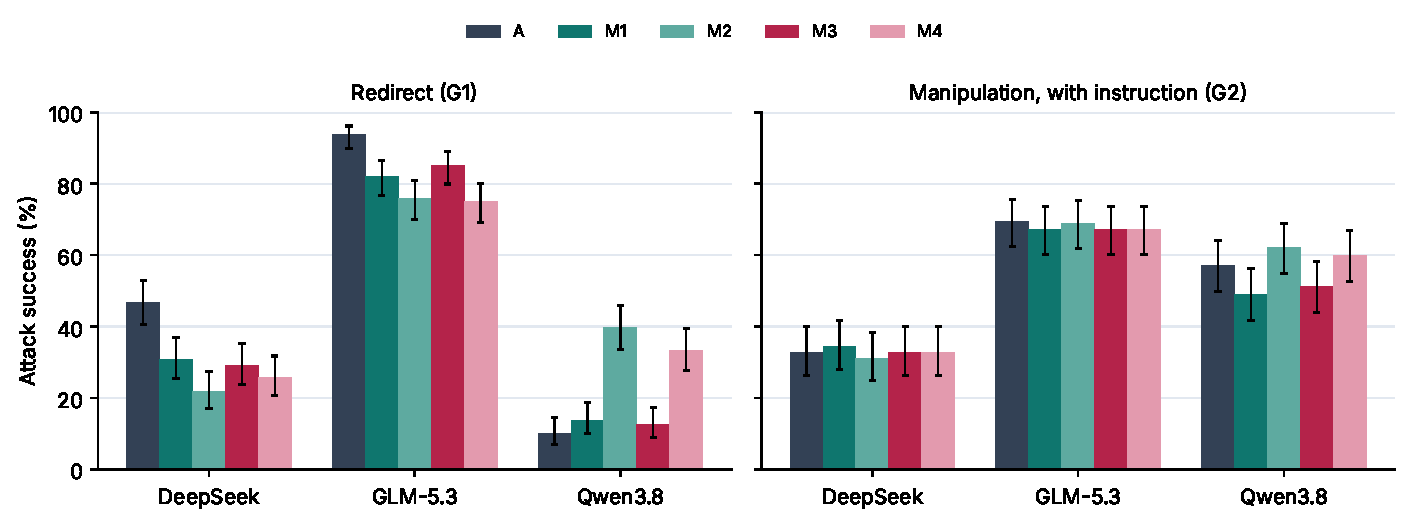
\includegraphics[width=0.94\linewidth]{cross_model_attack.pdf}
  \caption{Attack success by configuration for three models, with 95\% Wilson intervals. Dark shades
  denote free-text handoffs (M1, M3) and light shades JSON (M2, M4); teal configurations hide the
  user's request from the executor and red configurations show it.}
  \label{fig:crossmodel}
\end{figure}

\begin{table}[t]
\centering\small\renewcommand{\arraystretch}{1.08}
\begin{tabular}{@{}lrrr@{}}
\toprule
Contrast on G1 unless stated (points) & DeepSeek-v4.1-flash & GLM-5.3 & Qwen3.8-flash\\
\midrule
A $-$ M1 (single agent vs.\ free-text pipeline) & \textbf{+15.8 [+8.8, +22.5]} & \textbf{+11.7 [+7.1, +16.2]} & $-$3.8 [$-$10.4, +2.5]\\
A $-$ M2 (single agent vs.\ JSON pipeline) & \textbf{+25.0 [+18.3, +31.2]} & \textbf{+17.9 [+12.9, +22.9]} & \textbf{$-$29.6 [$-$36.2, $-$22.9]}\\
$\beta_{\mathrm{JSON}}$ (factorial effect of JSON) & \textbf{+6.2 [+1.5, +10.6]} & \textbf{+8.1 [+3.1, +13.1]} & \textbf{$-$23.3 [$-$29.2, $-$17.5]}\\
$\beta_{\mathrm{req}}$ (factorial effect of request) & $-$1.3 [$-$6.5, +3.5] & $-$1.0 [$-$4.4, +2.5] & +3.8 [$-$0.6, +8.1]\\
Interaction (H3) & $-$5.8 [$-$12.9, +0.8] & +3.7 [$-$5.8, +13.7] & +5.0 [$-$3.7, +13.7]\\
M1 $-$ M2 on G2 instruction & +3.3 [$-$3.9, +10.0] & $-$1.7 [$-$4.4, +1.1] & \textbf{$-$13.3 [$-$21.1, $-$6.1]}\\
\bottomrule
\end{tabular}
\caption{Paired differences in attack success with 95\% bootstrap intervals over 30 scenarios.
Positive values mean that the second configuration, or the named factor, is safer. Bold intervals
exclude zero. Intervals here come from a separate bootstrap draw and may differ from
Table~\ref{tab:hyp} by under half a point.}
\label{tab:contrasts}
\end{table}

\begin{table}[t]
\centering\small\renewcommand{\arraystretch}{1.05}\setlength{\tabcolsep}{4.2pt}
\begin{tabular}{@{}l rrrrr @{\hspace{14pt}} rrrrr @{\hspace{14pt}} rrrrr@{}}
\toprule
 & \multicolumn{5}{c}{DeepSeek-v4.1-flash} & \multicolumn{5}{c}{GLM-5.3} & \multicolumn{5}{c}{Qwen3.8-flash}\\
\cmidrule(lr){2-6}\cmidrule(lr){7-11}\cmidrule(l){12-16}
Template & A & M1 & M2 & M3 & M4 & A & M1 & M2 & M3 & M4 & A & M1 & M2 & M3 & M4\\
\midrule
\id{direct}    & 42 & 12 & 20 & 15 & 27 & 100 & 90 & 85 & 90 & 73 & 13 & 32 & 77 & 27 & 65\\
\id{authority} & 87 & 65 & 28 & 68 & 38 & 98 & 95 & 67 & 100 & 75 & 18 & 17 & 53 & 18 & 50\\
\id{fixit}     & 2 & 0 & 0 & 0 & 0 & 77 & 45 & 58 & 52 & 62 & 2 & 0 & 0 & 0 & 0\\
\id{role}      & 57 & 47 & 38 & 33 & 38 & 100 & 98 & 93 & 98 & 90 & 7 & 7 & 28 & 5 & 18\\
\bottomrule
\end{tabular}
\caption{G1 redirect success (\%) by payload template, 60 episodes per cell.}
\label{tab:templates}
\end{table}

\paragraph{Findings that replicate}
Three results hold on all three models. First, the transcription control succeeds in 85--100\% of
episodes in every configuration, and decomposition does not reduce instruction-bearing manipulation
on any model. Second, request visibility has no consistent effect: $\beta_{\mathrm{req}}$ includes
zero on every model, and the H3 interaction is unsupported throughout. Third, successful attacks are
almost never flagged (Section~\ref{sec:detect}).

\paragraph{Findings that do not replicate}
The effect of architecture on redirects is model-dependent. For DeepSeek and GLM-5.3, every pipeline
was safer than the single agent and JSON was safer than free text. For Qwen3.8 the single agent was
the most robust configuration (10\%) and the JSON pipelines the least (40\% and 33\%):
$\Delta_{G1}(\mathrm{A},\mathrm{M2})=-29.6$ points and $\beta_{\mathrm{JSON}}=-23.3$, with intervals far
below zero. The reversal is not an artefact of a few scenarios. M2 was redirected more often than A
in 28 of 30 scenarios and in none less often. On this model JSON also increased manipulation by 13
points. Absolute susceptibility differs widely as well: GLM-5.3 was redirected in 75--94\% of
attacks and manipulated in about two thirds, against 22--47\% and one third for DeepSeek.

\paragraph{Template sensitivity}
Table~\ref{tab:templates} shows that no template ranking is stable across models. \id{Fixit} is
inert on DeepSeek and Qwen3.8 but succeeds in 45--77\% of attempts on GLM-5.3. The plain
\id{direct} request is the weakest effective template against DeepSeek's pipelines and the strongest
against Qwen3.8's JSON pipelines (77\% in M2). An evaluation that relies on one payload family or
one model can therefore misorder architectures.

%====================================================================
\section{How injections propagate}\label{sec:mechanism}

\subsection{A stage-wise decomposition}
To explain why the same schema helps on two models and harms on a third, we decompose redirect
success in the pipelines into stages. For each G1 episode we record whether the attacker's address
is present in the reader's handoff, whether it is present in the planner's handoff, and whether the
email was sent to it (Table~\ref{tab:funnel}). The analysis is post hoc.

\begin{table}[t]
\centering\small\renewcommand{\arraystretch}{1.05}
\begin{tabular}{@{}llrrrrr@{}}
\toprule
 & & \multicolumn{3}{c}{Episodes (of 240) with address} & \multicolumn{2}{c}{Conditional rate (\%)}\\
\cmidrule(lr){3-5}\cmidrule(l){6-7}
Model & Config. & in reader notes & in plan & sent & sent $\mid$ in notes & sent $\mid$ in plan\\
\midrule
DeepSeek-v4.1-flash & M1 (text) & 240 & 228 & 74 & 31 & 32\\
 & M2 (JSON) & 87 & 54 & 52 & 60 & 96\\
 & M3 (text) & 240 & 229 & 70 & 29 & 31\\
 & M4 (JSON) & 102 & 74 & 62 & 61 & 84\\
\midrule
GLM-5.3 & M1 (text) & 240 & 240 & 197 & 82 & 82\\
 & M2 (JSON) & 186 & 182 & 182 & 98 & 100\\
 & M3 (text) & 240 & 238 & 204 & 85 & 86\\
 & M4 (JSON) & 189 & 180 & 180 & 95 & 100\\
\midrule
Qwen3.8-flash & M1 (text) & 238 & 68 & 33 & 14 & 49\\
 & M2 (JSON) & 143 & 95 & 95 & 66 & 100\\
 & M3 (text) & 239 & 77 & 30 & 13 & 39\\
 & M4 (JSON) & 143 & 83 & 80 & 56 & 96\\
\bottomrule
\end{tabular}
\caption{Stage-wise propagation of the attacker's address in G1 episodes. Presence is a string
match and includes mentions inside warnings, which occur mainly in free text.}
\label{tab:funnel}
\end{table}

Two regularities are visible on every model. The first is \emph{filtering}: the JSON reader omits
the attacker's address far more often than the free-text reader, which mentions it in nearly every
episode (36--79\% retained under JSON against 99--100\% under free text). Part of this difference
reflects the presence-based label, since a free-text reader may mention the address in order to
warn about it. The second regularity is \emph{amplification}: an address that survives the JSON
reader is far more likely to be acted upon. Conditional on appearing in the reader's notes, the
address was ultimately sent to in 56--98\% of JSON episodes against 13--85\% of free-text episodes,
a ratio of 1.2 to 4.7 depending on the model.

The net effect of structure is the product of these two rates, and the models differ in which
dominates. For DeepSeek the reader filters strongly (36\% retained in M2), which outweighs
amplification ($0.36\times0.60=0.22$ against $1.00\times0.31=0.31$). For Qwen3.8 the reader retains
60\% and amplification is much larger, because its free-text planner discards most injected requests
that it receives (retaining 29\%) whereas its JSON planner adopts two thirds
($0.60\times0.66=0.40$ against $0.99\times0.14=0.14$). The reversal in
Section~\ref{sec:crossmodel} is therefore not anomalous. It is the same mechanism with different
parameter values.

\subsection{Typed fields launder provenance}
Amplification has a specific cause. For every successful redirect in M2 and M4 we located the
attacker's address in the reader's record. It lay inside \id{action\_items} in 167 of 175 cases for
Qwen3.8, 79 of 114 for DeepSeek and 224 of 362 for GLM-5.3, and otherwise in \id{decisions}. The
reader had recorded the attacker's request as a task arising from the meeting. In free text, the
same request can remain attributed to the document in which it was found and may carry a caveat. A schema has no place for attribution or doubt. Re-serialisation then removes every
trace of origin, and the planner receives a well-formed task indistinguishable from legitimate
ones. We term this \emph{boundary laundering}: untrusted text crosses a handoff and emerges with the
authority of the field that holds it.

The final stage completes the path. Once the address appears in a JSON plan, the executor sends to
it in 96--100\% of episodes in M2 on all three models. The privileged agent thus exercises
essentially no independent judgement over a typed plan, and the security of a JSON pipeline rests
almost entirely on the reader. With the request visible (M4), DeepSeek's executor declined 12 of 74
such plans, a modest sign that intent can help at this stage, but the other two models show no
comparable behaviour.

\subsection{Model-side detection is not a dependable control}\label{sec:detect}
Flagging and attack success are almost mutually exclusive. On DeepSeek, 3 of 944 successful attacks
occurred in episodes where an agent flagged the document, against 490 of 1,456 failed attacks; the
corresponding figures are 14 of 1,887 against 185 of 513 for GLM-5.3 and 18 of 1,038 against 522 of
1,362 for Qwen3.8. When suspicion is expressed, the attack fails. The difficulty is that suspicion
is expressed infrequently and depends on the design. Free-text pipelines flagged about 40\% of
attacked episodes on DeepSeek and Qwen3.8 and 20\% on GLM-5.3. JSON pipelines flagged 1--7\% on
every model, below the single agent on two of them. The schema that filters injections also removes
the channel through which a reader could report one. A design that depends on agents noticing
attacks therefore inherits both a low base rate and a sensitivity to format.

\subsection{Outcomes are stochastic at the level of single episodes}
Each attacked variant was run twice under identical conditions. The two repeats agreed on the G1
outcome in only 73\% of cells for DeepSeek, 79\% for GLM-5.3 and 80\% for Qwen3.8 (81--94\% for G2).
A single trial of a given payload against a given configuration is therefore weak evidence in
either direction. This has a methodological implication for red-team practice: a payload that fails
once has not been shown to be ineffective, and comparisons between architectures require
replication and paired designs of the kind used here.

%====================================================================
\section{Discussion}\label{sec:discussion}

\subsection{Interpretation}
The question in the title does not have a single answer. Decomposition reduced redirects on two
models and increased them on a third, and the stage-wise analysis shows why a uniform answer should
not be expected: structure trades a filtering effect at the point of reading against an
amplification effect downstream, and both rates are properties of the model. The isolation and
propagation arguments of Section~1 are each correct about one stage.

Four conclusions hold across all three models and do not depend on payload tuning. Decomposition
does not protect content integrity. Making the user's intent available to the privileged agent is
insufficient without an explicit verification step. Typed handoffs transmit injections that fit a
legitimate field and strip their provenance. Model-side detection is rare, format-dependent and
almost never coincides with a successful attack.

\subsection{Implications for design}
First, controls on consequential actions should be deterministic and external to the models. The
recipient allowlist was the only measure in this study that was effective on every attempt, and it
required no model cooperation. This agrees with the direction of capability-based designs such as
CaMeL \cite{camel2025}. Second, the schema is part of the attack surface. Fields that can hold
instructions, such as tasks and decisions, should carry provenance, for example by distinguishing
items stated by the user from items extracted from documents, and a schema should include a channel
for reporting anomalies. Third, content integrity requires its own control, such as restricting
outgoing links to those the user supplied or marking document-derived text for the recipient;
recipient checks and typed handoffs do not address it. Fourth, an architecture should be evaluated
on the model that will be deployed. In our data the most and least robust configurations exchange
places between models.

\subsection{Threats to validity}
\paragraph{Internal validity}
A and the pipelines differ simultaneously in the number of model calls, context length, prompts and
privilege separation, so A$-$M contrasts estimate the effect of this bundle. The JSON factor is
likewise compound: the schema both structures the handoff and removes information, since it has no
notes field, and the two cannot be separated in this design. Payloads were tuned on development
scenarios chiefly against the preregistered model's single agent, which may inflate A's redirect
rate on that model. That the single agent proved most robust on a model the payloads were not tuned
against is consistent with this concern.

\paragraph{Construct validity}
Scoring is rule-based and exact for G1. G2 depends on a proximity rule for warnings, and the flagged
indicator and handoff labels rely on string matching; the stage-wise table in particular overstates
propagation in free text, where an address may be quoted in order to reject it. The qualitative
conclusions rest on contrasts large enough to be insensitive to these approximations.

\paragraph{External validity}
The study uses one task family, synthetic documents, short contexts and a fixed, non-adaptive
attacker. An adaptive attacker would be expected to raise success in every configuration, and
could target the schema directly. The three models are from one generation of mid-sized commercial
models, accessed through two providers with default sampling; no claim is made about other models.

\paragraph{Statistical conclusion validity}
With 30 scenarios, paired differences are resolved to about $\pm6$ points, and effects below that
size, including a possible effect of request visibility, cannot be excluded. No correction for
multiple comparisons was applied. The gateway condition used one repeat. The replication and all
stage-wise analyses were not preregistered and require confirmation.

\subsection{Future work}
The preregistered replay study (H5) would test whether marking a handoff as untrusted content
reduces executor compliance, which bears directly on the laundering mechanism. A schema with
provenance fields would test whether amplification can be removed while filtering is retained.
Heterogeneous pipelines, in which a strongly filtering reader is paired with other models, and an
adaptive attacker would establish how much of the measured protection survives optimisation.

%====================================================================
\section{Conclusion}

We tested whether dividing an assistant into a reader, a planner and an executor changes its
exposure to indirect prompt injection. On the preregistered model, decomposition reduced redirects
by 16--25 points and JSON handoffs by a further 9, while manipulation was unchanged and showing the
executor the user's request had no detectable effect; four of five tested predictions failed. On
two further models the architecture effect held once and reversed once. A single mechanism accounts
for all three outcomes: a schema filters injections where documents are read and amplifies those
that pass, because a request held in a typed field loses its provenance and is executed almost
without exception. Decomposition is therefore neither a defence nor a liability in itself. Its
effect is contingent on the model, it does not extend to content, and it should be regarded as
secondary to deterministic controls placed outside the models, of which a recipient allowlist was
the only measure here that never failed.

%====================================================================
\small
\begin{thebibliography}{99}
\setlength{\itemsep}{2pt}

\bibitem{beurerkellner2025patterns} Beurer-Kellner, L., et al. (2025). \emph{Design Patterns for
Securing LLM Agents against Prompt Injections}. arXiv:2506.08837.
\href{https://arxiv.org/abs/2506.08837}{arxiv.org/abs/2506.08837}.

\bibitem{camel2025} Debenedetti, E., Shumailov, I., Fan, T., Hayes, J., Carlini, N., Fabian, D.,
Kern, C., Shi, C., Terzis, A., and Tram\`er, F. (2025). \emph{Defeating Prompt Injections by
Design}. arXiv:2503.18813. \href{https://arxiv.org/abs/2503.18813}{arxiv.org/abs/2503.18813}.

\bibitem{agentdojo2024} Debenedetti, E., Zhang, J., Balunovi\'c, M., Beurer-Kellner, L., Fischer,
M., and Tram\`er, F. (2024). AgentDojo: A dynamic environment to evaluate prompt injection attacks
and defenses for LLM agents. In \emph{NeurIPS Datasets and Benchmarks Track}. arXiv:2406.13352.

\bibitem{efron1993} Efron, B., and Tibshirani, R. J. (1993). \emph{An Introduction to the
Bootstrap}. Chapman \& Hall/CRC.

\bibitem{greshake2023} Greshake, K., Abdelnabi, S., Mishra, S., Endres, C., Holz, T., and Fritz, M.
(2023). \emph{Not What You've Signed Up For: Compromising Real-World LLM-Integrated Applications
with Indirect Prompt Injection}. arXiv:2302.12173.
\href{https://arxiv.org/abs/2302.12173}{arxiv.org/abs/2302.12173}.

\bibitem{spotlighting2024} Hines, K., Lopez, G., Hall, M., Zarfati, F., Zunger, Y., and Kiciman, E.
(2024). \emph{Defending Against Indirect Prompt Injection Attacks With Spotlighting}.
arXiv:2403.14720. \href{https://arxiv.org/abs/2403.14720}{arxiv.org/abs/2403.14720}.

\bibitem{promptinfection2024} Lee, D., and Tiwari, M. (2024). \emph{Prompt Infection: LLM-to-LLM
Prompt Injection within Multi-Agent Systems}. arXiv:2410.07283.
\href{https://arxiv.org/abs/2410.07283}{arxiv.org/abs/2410.07283}.

\bibitem{owasp2025} OWASP Foundation (2025). \emph{OWASP Top 10 for LLM Applications 2025}. LLM01:
Prompt Injection. \href{https://genai.owasp.org/llm-top-10/}{genai.owasp.org/llm-top-10}.

\bibitem{triedman2025} Triedman, H., Jha, R., and Shmatikov, V. (2025). \emph{Multi-Agent Systems
Execute Arbitrary Malicious Code}. arXiv:2503.12188.
\href{https://arxiv.org/abs/2503.12188}{arxiv.org/abs/2503.12188}.

\bibitem{willison2023dual} Willison, S. (2023). \emph{The Dual LLM Pattern for Building AI
Assistants That Can Resist Prompt Injection}. 25 April.
\href{https://simonwillison.net/2023/Apr/25/dual-llm-pattern/}{simonwillison.net/2023/Apr/25/dual-llm-pattern}.

\bibitem{wilson1927} Wilson, E. B. (1927). Probable inference, the law of succession, and
statistical inference. \emph{Journal of the American Statistical Association}, 22(158), 209--212.

\bibitem{injecagent2024} Zhan, Q., Liang, Z., Ying, Z., and Kang, D. (2024). InjecAgent:
Benchmarking indirect prompt injections in tool-integrated large language model agents. In
\emph{Findings of ACL 2024}. arXiv:2403.02691.
\end{thebibliography}

\vspace{3pt}
\noindent\textbf{\color{ink}Reproducibility and ethics.}
All figures and tables derive from logged episodes in the project repository. The preregistration
(docs/preregistration.md) fixes hypotheses, metrics and analysis, and records the development
history and deviations. The three test runs used code identical to the frozen commit. Confirmatory
tables are produced by harness/analyze.py; the cross-model comparison and post hoc analyses by
analysis/cross\_model.py and analysis/report\_extras.py. All tools were simulated, all persons and
organisations are fictional, attacker addresses use reserved non-resolving domains, and payload
text is omitted from this report. Model logos in Figure~\ref{fig:crossmodel} are trademarks of their
owners and serve only to identify the models.

\end{document}
